\subsection{The MP-SRP-PHAT algorithm}

The MP-SRP-PHAT implementation steps are described in Fig. \ref{fig:systemimplementaiton}. The algorithm is basically the same as the normal SRP-PHAT algorithm discussed before, with the only change happening at the last step where the minimum power from the localization cones is considered, instead of summing the power from all the cones.  % there exist methods to improve the efficiency of the algorithm but this is not the focus of this work. \footnote{Dmochowski and Benesty \cite{dmochowski2007generalized} present a method which improve the full map search}. 
The computational complexity of the algorithm and the practical implementation details are discussed in this section. The delays across the microphones for each search location on the search map are computed in advance, stored in memory and fed to the algorithm which correspond to the `Compute array delays' system block in the figure, therefore this step will not be considered computational load. Upon running the algorithm, first of all the computer reads the stored .wav files into memory. The signal cross correlation between each pair of microphones are then computed. This step is the `GCC-PHAT' block in Fig. \ref{fig:systemimplementaiton}. The `SRP' system block is related to the array steering for each of the search location $(\theta,\phi)$. This step looks up the delay table corresponding the $(\theta,\phi)$ for each microphone pair, and saves the corresponding power associated with that delay and that pair into an array ($P_{all}$). So $P_{all}$ contains 6 power values for each location on the search map. The minimum power then selected from $P_{all}$ the 6 power values for each of the locations $(\theta,\phi)$ and this value is stored in the result array\footnote{One thing to note is that there is a limit to the granularity of the $(\theta,\phi)$, the achievable angular resolution. The angular resolution of localization is in fact not linear, as shown in \ref{fig:ang_res}(A delay of one sample does not always correspond to the same change in degree). The SRP-MAP can then be plotted by computing the delays sequentially for a particular angular resolution. However, these delays might be fractional. Since, the values of fractional delays cannot be picked from the cross-correlation array \textit{R}, these delays are rounded. One way to increase the angular resolution is to increase the sample rate. That way even if fractional delays are encountered, they would be less erroneous. Another way is to apply interpolation to find the value at the fractional delays. For the purpose of this thesis, the interpolation techniques are not considered.}.

\begin{figure}[!ht]
    \centering
    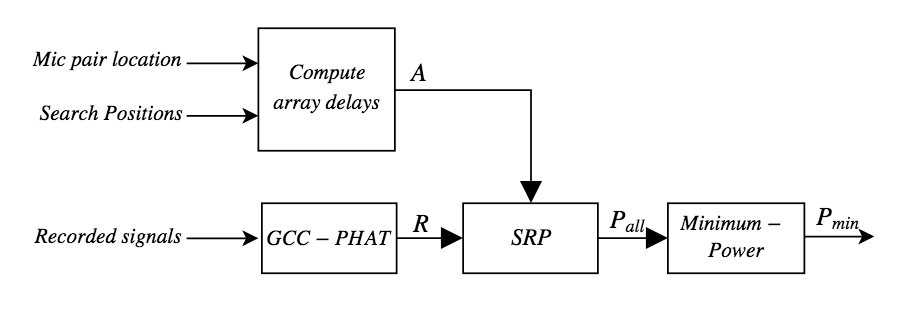
\includegraphics[width=1\textwidth]{Figures/system1.png}
    \caption{Overall localization algorithm}
    \label{fig:systemimplementaiton}
\end{figure}

The MP-SRP-PHAT algorithm combines beamforming techniques with cross correlation methods for several pairs of microphones. While the beamforming part does not depend on the size of the input data, it might become a challenge memory wise to store the delay for each search position. The most computationally demanding part of the algorithm is definitely the cross-correlation part. By performing the cross-correlation in the frequency domain, i.e by using the cross-spectrum between pairs of microphones, better averaging of the stationary sources are obtained as well as better efficiency compared to time domain cross-correlation ($\mathcal{O}(n^2)$). The cross-spectrum computation is described in Fig. \ref{fig:crossspectrumsystem}.
\begin{figure}[H]
    \centering
    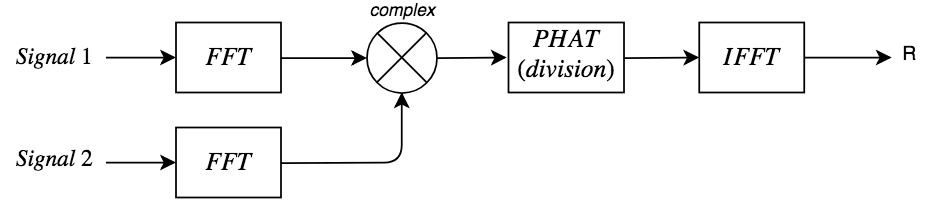
\includegraphics[width=1\textwidth]{Figures/crossspectra.png}
    \caption{Cross spectrum between two signals}
    \label{fig:crossspectrumsystem}
\end{figure}
%Dmochowski and Benesty \cite{dmochowski2007generalized} detailed the number of computation needed for the GCC-PHAT part,
Note that not the entire R computed this way is important for the purpose of localization. This is because only a finite number of samples can exist between two microphones, say \textit{d}. \textit{d} depends on the array aperture size as well as the sample rate. Delays$\gt$\textit{d} could not have been measured by the microphone array. For this reason the R is cropped down to \textit{d}. Since, the signals arriving at two microphones can be either in front or behind each other, both the first and last \textit{d} samples of R are taken. The worst-case complexity of the cross-spectrum computation is listed below, with \textit{n} being the number of input samples (signal length) in the algorithm. 
\begin{center}
  \begin{tabular}{ |c | c | }
    \hline
    Operation  & Worst-case Complexity \\ \hline
    FFT  & $\mathcal{O}(n\log{}n)$  \\ \hline
    Complex Multiplication  & $\mathcal{O}(n)$  \\ \hline
    PHAT (Division)  & $\mathcal{O}(n)$  \\ \hline
    IFFT  & $\mathcal{O}(n\log{}n)$  \\
    \hline
  \end{tabular}
\end{center}
The SRP block is also computationally heavy, however, it does not scale with the number of samples but rather with the number of locations to look up in the SRP block. %Dmochowski and Benesty \cite{dmochowski2007generalized} also proposed a more efficient way to perform the SRP.
Therefore the overall algorithm complexity scales with the FFT complexity $\mathcal{O}(n\log{}n)$ when n is the number of samples. %When n is small the FFT is negligible to the number of delay lookups.
\begin{figure}[!ht]
    \centering
    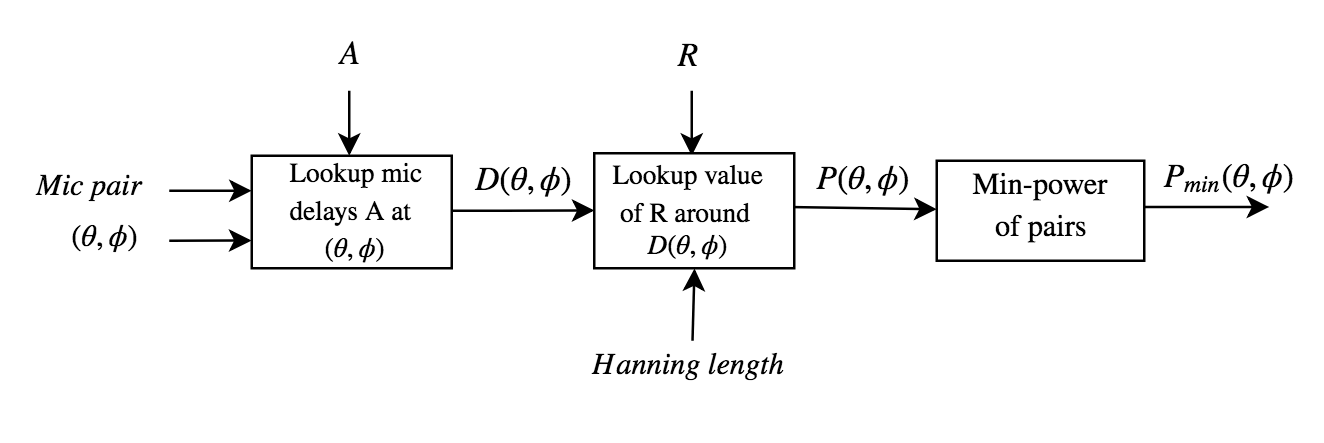
\includegraphics[width=1\textwidth]{Figures/system2.png}
    \caption{SRP block + Minimum Power}
    \label{fig:system2}
\end{figure}
%Table \ref{tab:extime} gives a measure of the execution time of the minimum SRP-PHAT script. 
%\begin{center}
%  \begin{tabular}{ c | c | c |}
%    \cline{2-3}
%    \multicolumn{1}{c|}{} & \multicolumn{2}{ c| }{Execution time} \\ \cline{2-3}
%    \hline
%    \multicolumn{1}{|c|}{signal lengths (seconds)}   & thinkpad i5 & Macbook 2012  \\ \cline{1-3}
%    \multicolumn{1}{|c|}{10}  &  &    \\ \cline{1-3}
%    \multicolumn{1}{|c|}{100} & &     \\ \cline{1-3}
%    \multicolumn{1}{|c|}{1000}  & &   \\
%    \hline
%  \end{tabular}
%  \label{tab:extime}
%\end{center}
Memory wise, the function computing the delays at each pair of microphones in the array can be expensive depending on the localization resolution used and the number of microphone pairs. If 1$\degree$ resolution is used $360*180=64800$ delays are computed for a pair of microphones. For 6 microphone pairs,$360*180*6=388800$.  Using type float64 (8 bytes), the delay table is  $360*180*6*8=3110400$ = 3.11 MB. However, if high resolution is needed, i.e suppose 0.1$\degree$ resolution $3600*1800=6480000$ delays are computed. For 6 microphones,$3600*1800*6=38880000$.  Using type float64 (8 bit), the delay table is  $3600*1800*6*8=311040000$ = 311.04 MB.